\subsection{RL \& TOC-Based Simulation
Model}\label{rl-toc-based-simulation-model}

The TOC \& RL-based simulation model was also built upon the virtual
environment established in Section 4.1. Fifty variables were used to
represent the state space of the environment at each time step \(t\),
i.e.,
\(\mathcal{S =}\left\{ H_{i_{t}}^{OB},H_{i_{t}}^{CB},H_{i_{t}}^{SB},W_{i_{t}}^{CB},W_{i_{t}}^{SB}\ |\ h \in \mathbb{Z,\ }w = 0,\ 1,\ \ldots,\ 13 \right\}_{i = 1}^{I = 10}\).
The true buffer levels \((h)\) can take any integer value, being
negative when demand exceeds the buffer reference level, particularly
for SB. The true values of work-in-process \((w)\) can range from 0 to
13, with 13 occurring when all resources \(j\) in the longest production
route are occupied (see \colorbox{yellow!40}{\hyperref[_Ref187516873]{Figure 2}} and
Table S1). This state space informs the agent, which selects the number
of products to produce during the replenishment interval from a set of
\colorbox{yellow!40}{210} possible actions, i.e.,
\(\mathcal{A(S) =}\left\{ M_{i_{t}}\ |\ m = 0,\ 1,\ldots,\ 20 \right\}_{i = 1}^{I = 10}\).
This decision is made autonomously and is not explicitly modeled by
Equation 17. The quantity of each product to be produced ranges from 0
to \colorbox{yellow!40}{20}, with 0 representing the decision to produce nothing. The
maximum limit of \colorbox{yellow!40}{20} was set based on the highest order size
observed in the TOC-based model after \colorbox{yellow!40}{xx} replications and then
duplicated. The production sequence follows Equation 15, but similarly
to the TOC-based model, it is assumed that
\(\left( \rho_{i} - c_{i} \right) = 1\) when defining \(\tau_{i}\) in
Equation 10, since the original work by Atwater and Chakravorty
(\colorbox{yellow!40}{2002}) does not take into account the revenue and variable costs of
the products sold. The release of orders follows Equation 19. These
relationships are illustrated in \colorbox{yellow!40}{\hyperref[_Ref187516938]{Figure
5}}.

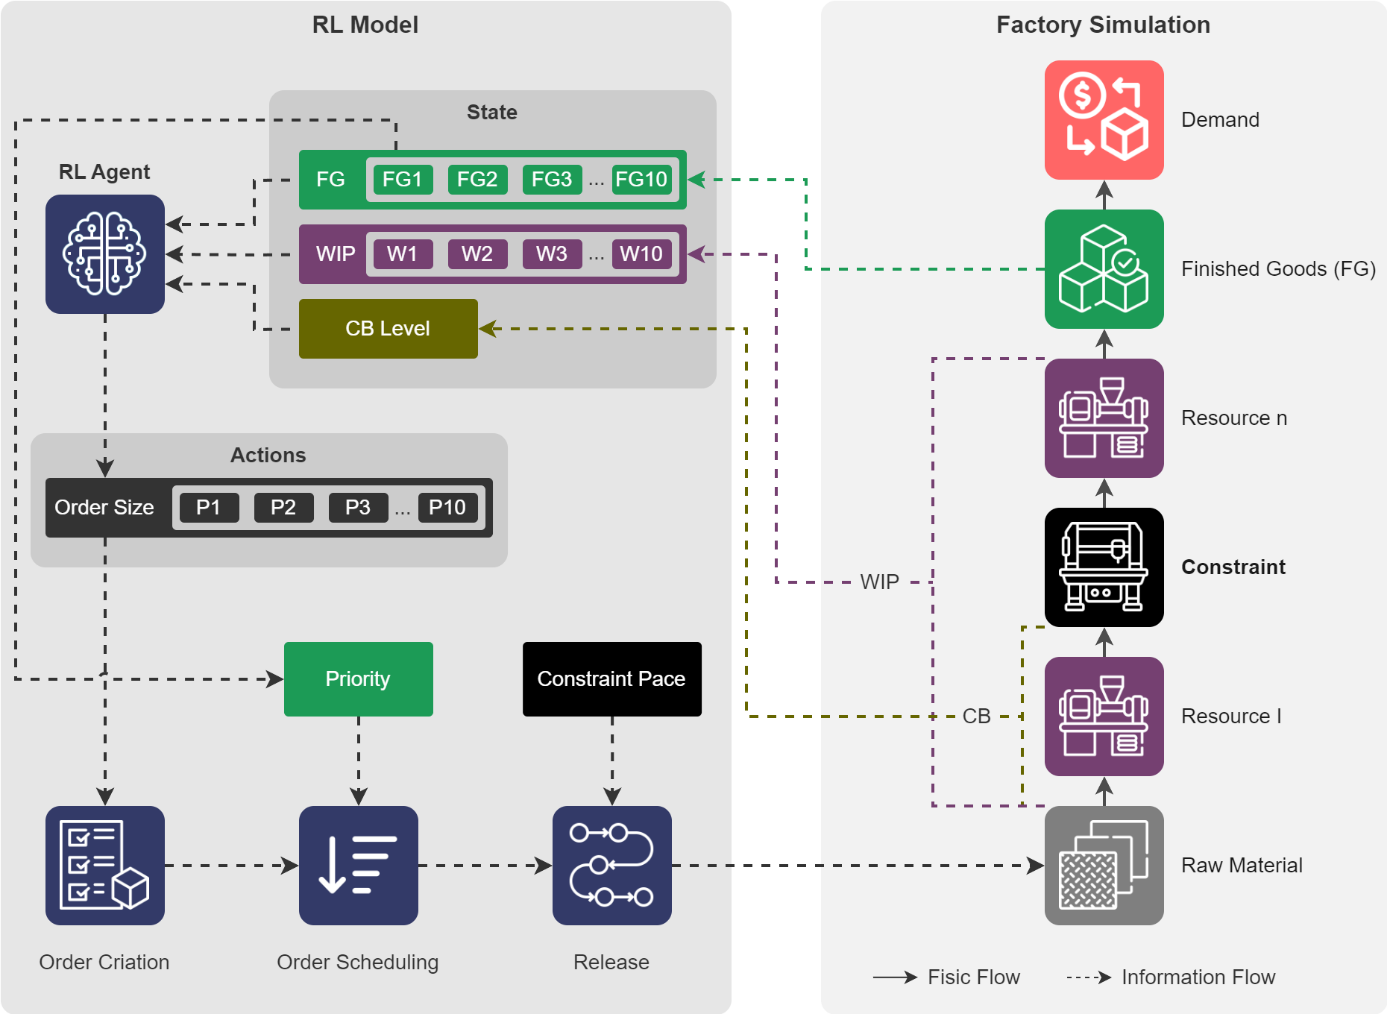
\includegraphics[width=6.29514in,height=4.60302in,alt={Diagrama Descrição gerada automaticamente}]{figures/fig05.png}

\protect\phantomsection\label{_Ref187516938}{}\colorbox{yellow!40}{Figure 5. Outline of
the RL \& TOC-based simulation model.}

The agent receives a numerical reward \(R_{t + 1}\) as a result of its
action (Sutton and Barto, 2018). Two of the performance measures from
the TOC are implicitly used as penalty subfunctions within the following
reward function:

\begin{equation}
R_{t + 1}\  = \frac{1}{I}\sum_{\forall i}^{}{1 - P_{i_{t + 1}}^{\tau} - P_{i_{t + 1}}^{W^{SB}} - P_{i_{t + 1}}^{H^{CB}} - P_{i_{t + 1}}^{H^{SB}}}.
\tag{20}
\end{equation}

The first of these measures is throughput \((\tau)\), which, due to the
original work by Atwater and Chakravorty (\colorbox{yellow!40}{2002}) lacking information
for its calculation, is treated as a penalty for lost sales (\colorbox{yellow!40}{cf.
Reference}). In other words, whenever the demand for a product exceeds
its current level in the SB, the system immediately fails to make a sale
and, consequently, cannot convert inventory into throughput (\colorbox{yellow!40}{cf.,
Reference}). This penalty is incurred whenever the SB level is negative.
Equation 21 outlines this condition, weighted by a factor of 0.3, which
gives greater importance to this penalty:

\begin{equation}
P_{i_{t + 1}}^{\tau} = \left\{ \binom{0.3H_{i_{t}}^{SB}\ }{0\ \ \ \ \ \ \ \ \ \ \ \ }\binom{if\ H_{i_{t}}^{SB} < 0}{if\ H_{i_{t}}^{SB} \geq 0} \right.\ .
\tag{21}
\end{equation}

The second measure is inventory \(\mathcal{(i)}\), which in the model is
represented by the quantity of items rather than monetary values, for
the same reason as throughput. Inventory is divided into three penalty
subfunctions, each squared, to amplify the impact of larger values
(\colorbox{yellow!40}{cf., Reference}). The first subfunction penalizes work-in-process
throughout the system, \(P_{i_{t + 1}}^{W^{SB}}\). The second penalizes
the level of the CB, \(P_{i_{t + 1}}^{H^{CB}}\), while the third
penalizes the number of items in the SB, \(P_{i_{t + 1}}^{H^{SB}}\). The
overall goal is to prevent lost sales while maintaining the lowest
possible inventory level (\colorbox{yellow!40}{cf., Schragenheim, 2010b}). For this
reason, the weight is smaller in Equation 24, while the other equations
have equal weights.

\begin{equation}
P_{i_{t + 1}}^{W^{SB}} = \left( 0.02W_{i_{t}}^{SB} \right)^{2};
\tag{22}
\end{equation}

\begin{equation}
P_{i_{t + 1}}^{H^{CB}} = \left( 0.02H_{i_{t}}^{CB} \right)^{2};
\tag{23}
\end{equation}

\begin{equation}
P_{i_{t + 1}}^{H^{SB}} = \left( 0.01H_{i_{t}}^{SB} \right)^{2};
\tag{24}
\end{equation}

In the RL \& TOC-based simulation model, the natural event that
determines the length of each simulation run, or episode in
reinforcement learning terminology (\colorbox{yellow!40}{cf., Reference}), is the
\colorbox{yellow!40}{72}-hour replenishment interval \((\mathrm{\Delta}\varphi)\). By
incorporating the reward function (Equation 21) into the return function
(Equation 2) and assuming a discount factor \(\gamma = 0.0\), along with
rewards received at future time steps (\(k = 71\)), we can construct the
state value function (Equation 3), from which the agent can be trained
to seek the optimal policy, \(\pi_{*}\).

The algorithm used for training the optimal policy is PPO (\colorbox{yellow!40}{Schulman
et al., 2017}), implemented using the Stable Baselines 3 library
(\colorbox{yellow!40}{Raffin et al., 2021}), which employs neural networks to approximate
both the policy and the state-value function (\colorbox{yellow!40}{Russell and Norvig,
2010; Schulman et al., 2017}). A learning rate of
\(\epsilon = 0.0002\ \) (Equation 7) and a maximum number of 277,777
replications (or episodes) were used during training, with the virtual
environment being reset each time the return reached zero (\colorbox{yellow!40}{cf.
Reference}). The maximum number of episodes was set based on
{[}\colorbox{yellow!40}{define the reason}{]} (\colorbox{yellow!40}{cf., Reference}). Two criteria were
used to terminate the training process (\colorbox{yellow!40}{Reference}): (i) the maximum
number of episodes was reached, or (ii) return saturation occurred,
where the return remained stable over \colorbox{yellow!40}{xx} episodes.

From a computational perspective, the training process was completed in
2 hours, utilizing 15 machines running in parallel, each with the
following specifications: an i5-13450HX processor, 16 GB of RAM, and an
NVIDIA GeForce RTX 4050 graphics card. A \colorbox{yellow!40}{state-value of 0.996} was
achieved after 13,888 episodes, as shown in
\colorbox{yellow!40}{\hyperref[_Ref187516969]{Figure 6}}a. The behavior of penalty
subfunctions is also illustrated in \colorbox{yellow!40}{\hyperref[_Ref187516969]{Figure
6}}b-d.

\begin{figure}[htbp]
\centering
\begin{subfigure}[b]{\textwidth}
\centering
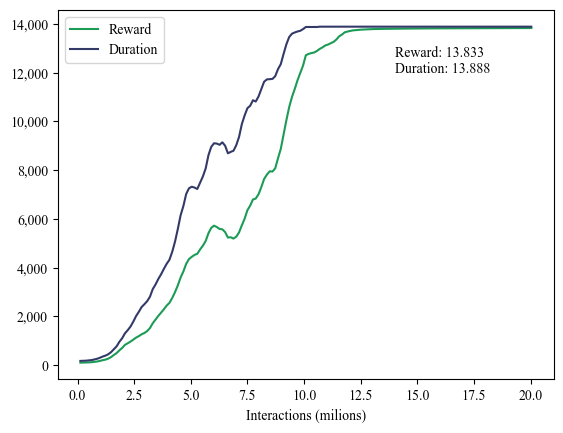
\includegraphics[width=\linewidth]{figures/fig06a.png}
\caption{}
\label{fig:sub:a}
\end{subfigure}
%
\begin{subfigure}[b]{0.48\textwidth}
\centering
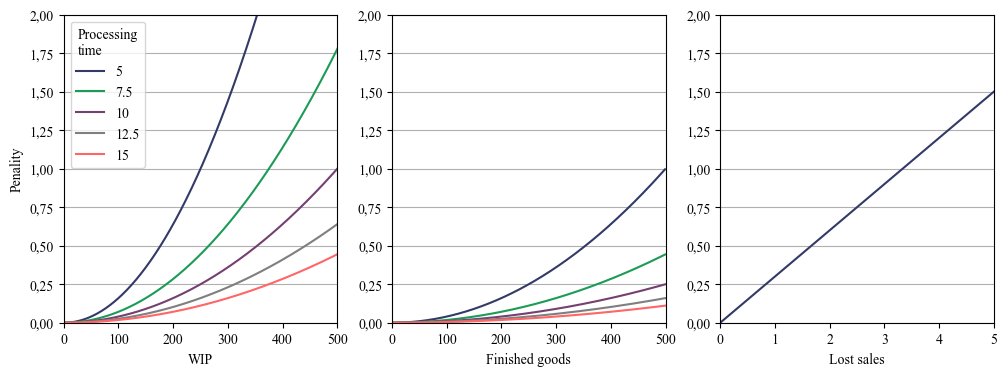
\includegraphics[width=\linewidth]{figures/fig06bcde.png}
\caption{}
\label{fig:sub:b}
\end{subfigure}
\begin{subfigure}[b]{0.48\textwidth}
\centering
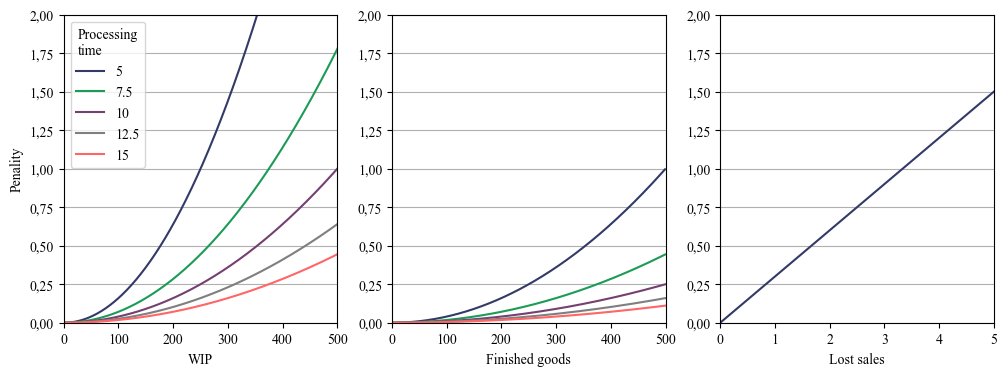
\includegraphics[width=\linewidth]{figures/fig06bcde.png}
\caption{}
\label{fig:sub:c}
\end{subfigure}
%
\begin{subfigure}[b]{0.48\textwidth}
\centering
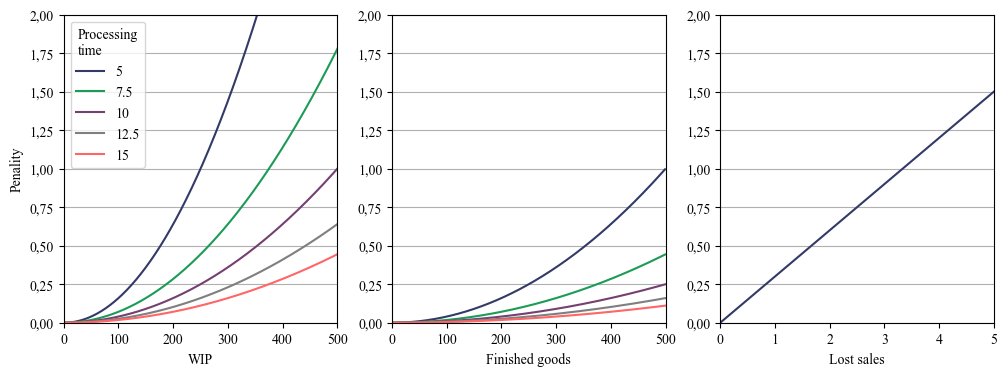
\includegraphics[width=\linewidth]{figures/fig06bcde.png}
\caption{}
\label{fig:sub:d}
\end{subfigure}
\begin{subfigure}[b]{0.48\textwidth}
\centering
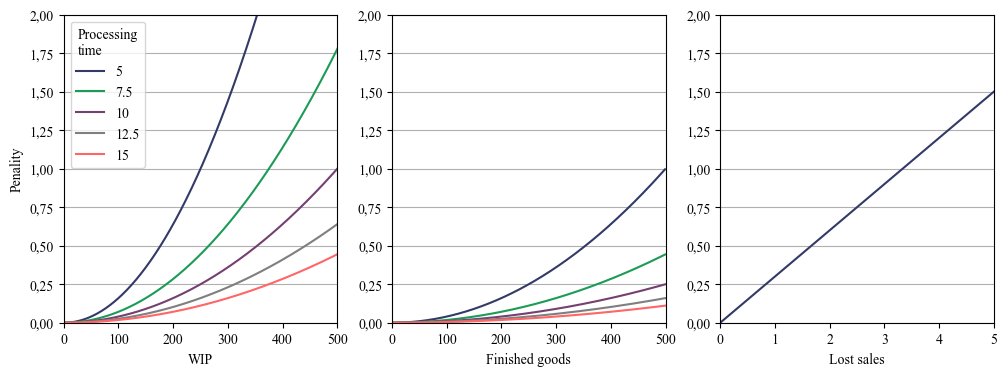
\includegraphics[width=\linewidth]{figures/fig06bcde.png}
\caption{}
\label{fig:sub:e}
\end{subfigure}
%
\caption{\protect\phantomsection\label{_Ref187516969}{}\colorbox{yellow!40}{Figure 6. Dynamic
behaviour of: (a) the return function; (b) the penalty subfunction for
lost sales; (c) the penalty subfunction for work-in-process; (d) the
penalty subfunction for the CB level; and (e) the penalty subfunction
for the SB level.}}
\end{figure}
